%\renewcommand{\chaptername}{Section}

\chapter{Introduction}
\label{chapt:intro}

This is the introduction, why we are doing this analysis

\section{Background} % (fold)

\Company does this as per Figure~\ref{fig:companypic} seen below.

%%[htbp] (here, top, bottom, page).  ! means no restriction for placement
%http://tex.stackexchange.com/questions/2275/keeping-tables-figures-close-to-where-they-are-mentioned help
\begin{figure}[!htbp]
    \centering
    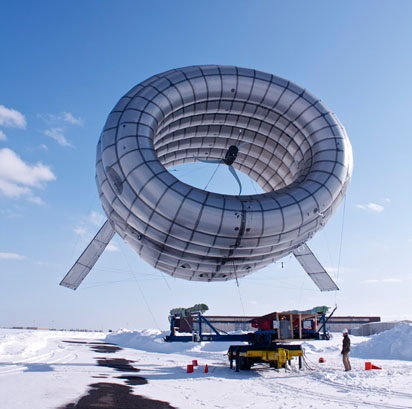
\includegraphics[width=0.6\textwidth]{companypic}
    \caption{Overview of the buoyant airborne technology}
    \label{fig:companypic}
\end{figure}


\section{Purpose}
The purpose of this report is to do this.
\begin{itemize}
    \item Do analysis on drum
    \item Development numerical algorithm for solving
\end{itemize}


\section{Scope} % (fold)

The scope of the report will be as follows.

\chapter{Preliminary Analysis}
The analysis process is discussed
\section{Simplifications}
The results were simplified to do.

\subsection{Equations}

The first equation that is presented , Equation~\ref{eq:statics}

\begin{equation}\label{eq:statics}
	%\frac{\partial (\rho\mathbf{v})}{\partial t} + \nabla \cdot (\rho \mathbf{v} \mathbf{v}) = -\nabla p + \nabla \cdot\mathbf{T} + \mathbf{f}. 
	\Sigma F_i=0	,	\Sigma	 M_0=0 
\end{equation} 


\chapter{Supplemental}
\subsection{Installation} % (fold)
LaTeX is based on open-source code, so it is available on most computing platforms as free software. If encounter some compiling problems after installation, please Google it. For example, MikTeX may complain about "mathtools.sty", a solution given on "StackExchange" is "The problem is that the package manager has somehow "desynchronized" (even though it's a fresh install). To fix it, run Miktex Package Manager as administrator---"Package Manager (Admin)". Go to Repository--Synchronize. When that completes, your TexWorks should automatically find the needed style files again."
\begin{itemize}
    \item Linux: TeXLive distribution. 
    \item MacOS: Mactex or TeXLive.
    \item Windows: MikTeX or TeXLive. 
\end{itemize}

Note: to use \LaTeX{}, you need a text editor for writing and editing ".tex" files. To open the ".tex" files in this template, you need a text editor which supports "UTF-8" encoding. Free options for different platforms are the following:
\begin{itemize}
    \item Linux: vim. 
    \item MacOS: TeXShop, Macvim.
    \item Windows: Texmaker, Gvim, Notepad++. 
\end{itemize}
% subsection Installation (end)

\subsection{Give a try} % (fold)
After downloading this template and installing a \LaTeX{} distribution. It's time to have a try:
\begin{itemize}
    \item Linux: run Compile.sh
    \item MacOS: run Compile.sh
    \item Windows: run Compile.bat
\end{itemize}

% subsection Give a try (end)

\subsection{Include math} % (fold)
\LaTeX{} realization of Equation~\ref{eq:N-S_equation} is something like this:
\begin{center}
    \small
    % Verbatim is used to show the actual latex comands and not complied
    \begin{verbatim}
    \begin{equationa}\label{eq:N-S_equation}
        \frac{\partial (\rho\mathbf{v})}{\partial t} +
        \nabla \cdot (\rho \mathbf{v} \mathbf{v}) =
        -\nabla p + \nabla \cdot\mathbf{T} + \mathbf{f}. 
    \end{equation}    
\end{verbatim}
\end{center}

\begin{equation}\label{eq:N-S_equation}
    \frac{\partial (\rho\mathbf{v})}{\partial t} + \nabla \cdot (\rho \mathbf{v} \mathbf{v}) = -\nabla p + \nabla \cdot\mathbf{T} + \mathbf{f}. 
\end{equation}    
% subsection Include math (end)

\subsection{Include Graphics} % (fold)
Note: inluding figures may seem to be scary by looking at the codes. However, the fact is that you only need to modify the names in each part, the rest are simply copy and paste. These codes are all available in the file "Useful Commands.txt".

Figure~\ref{fig:ITC_Q_Criteria} is an example for including a single figure.
\begin{center}
    \small
    \begin{verbatim}
        \begin{figure}[!htbp]
            \centering
            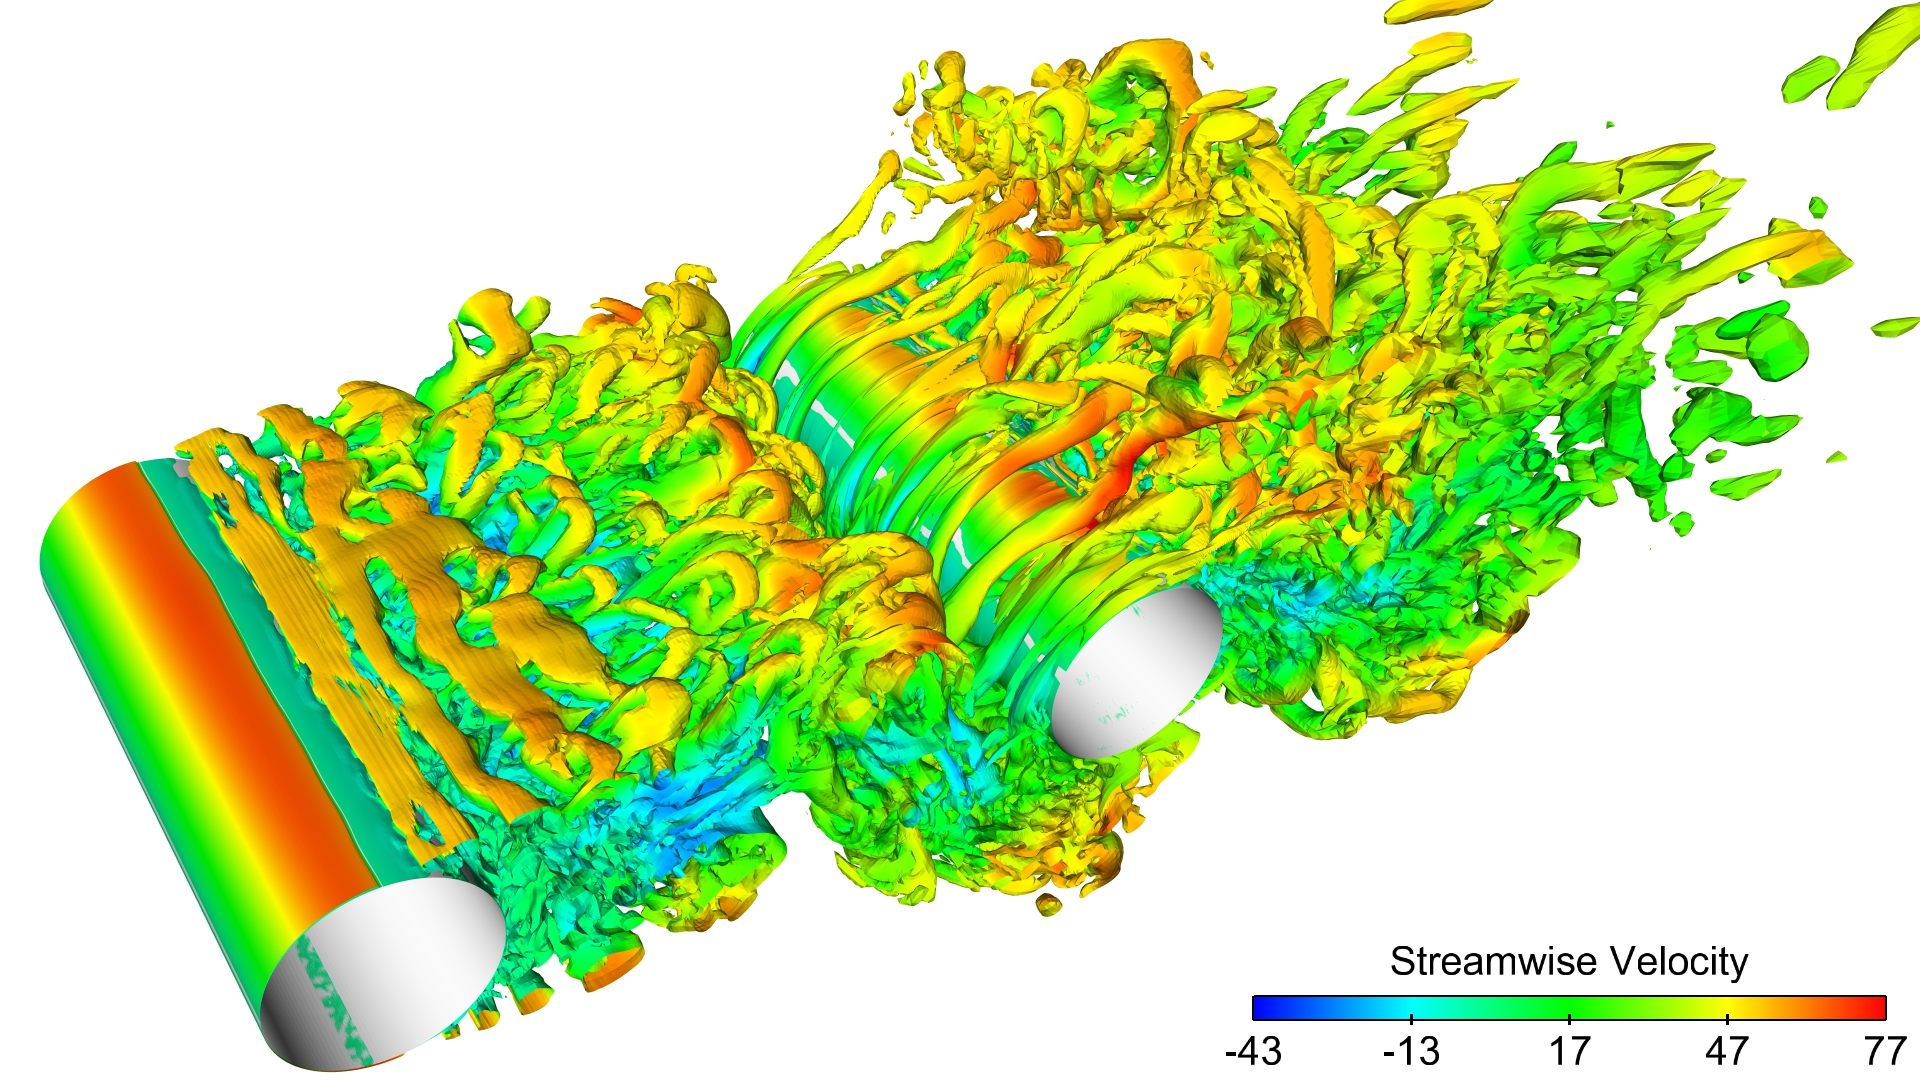
\includegraphics[width=0.45\textwidth]{ITC_Q_Criteria}
            \caption{An Example for including a single figure}
            \label{fig:ITC_Q_Criteria}
        \end{figure}
    \end{verbatim}
\end{center}

\begin{figure}[!htbp]
    \centering
    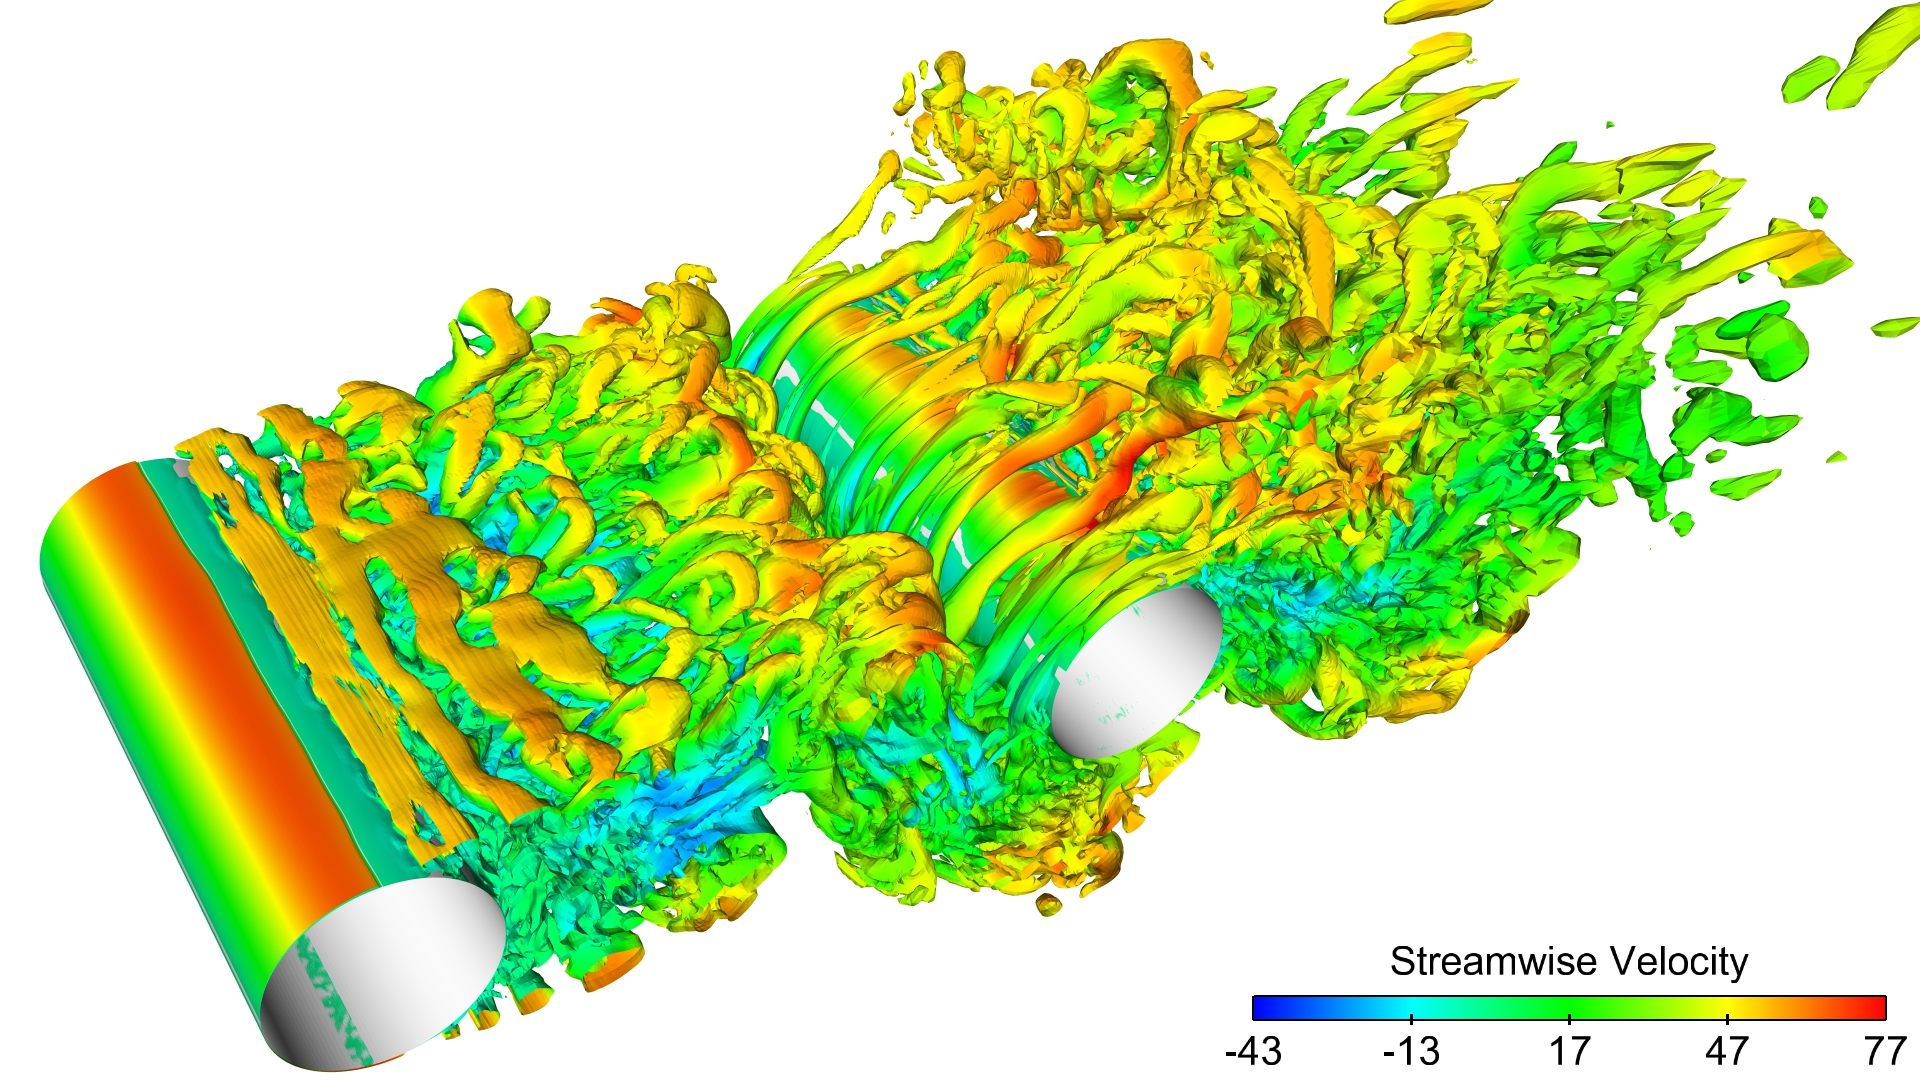
\includegraphics[width=0.45\textwidth]{ITC_Q_Criteria}
    \caption{An Example for including a single graph}
    \label{fig:ITC_Q_Criteria}
\end{figure}

Figure~\ref{fig:HC_OASPL} is an example for including multiple figuress. 
\begin{center}
    \small
    \begin{verbatim}
        \begin{figure}[!htbp]
            \centering
            \begin{subfigure}[b]{0.45\textwidth}
                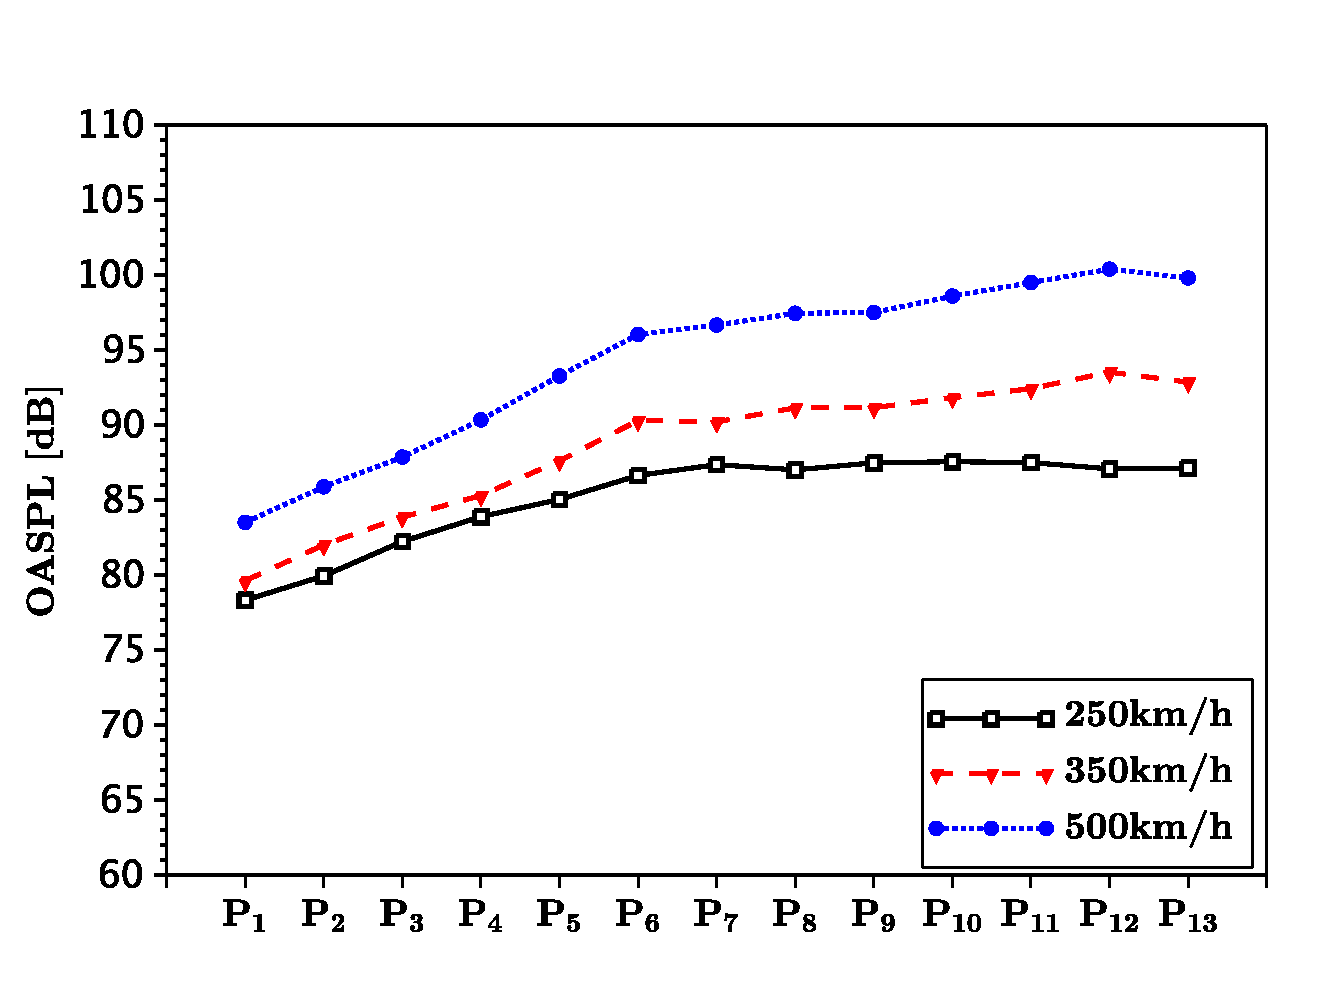
\includegraphics[width=\textwidth]{HC_OASPL_A}
                \caption{}
                \label{fig:HC_OASPL_A}
            \end{subfigure}%
            ~% add a small space
            \begin{subfigure}[b]{0.45\textwidth}
                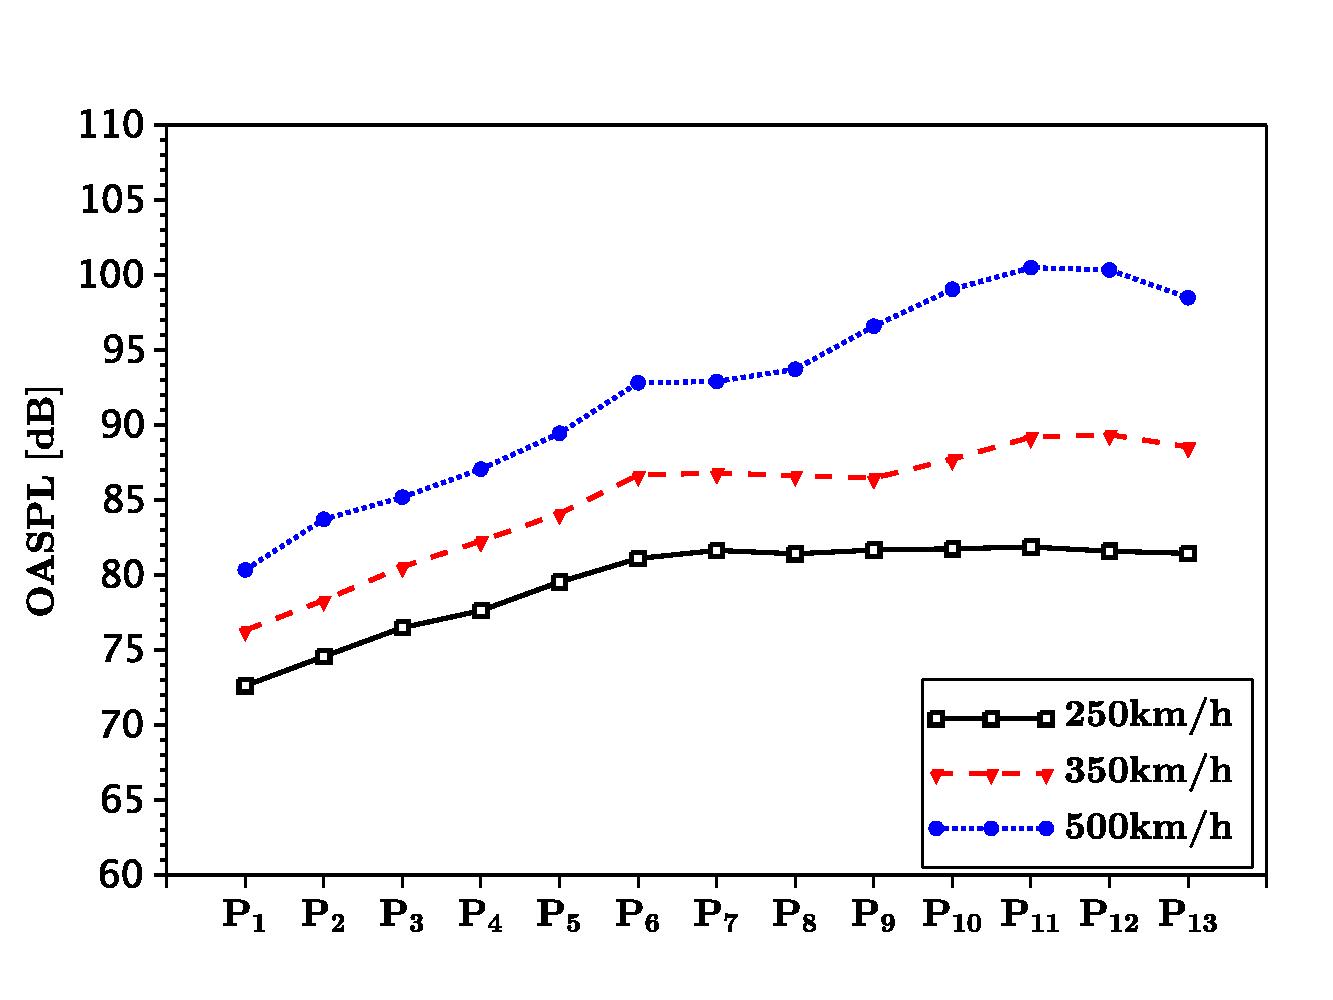
\includegraphics[width=\textwidth]{HC_OASPL_B}
                \caption{}
                \label{fig:HC_OASPL_B}
            \end{subfigure}%
            \\% change line
            \begin{subfigure}[b]{0.45\textwidth}
                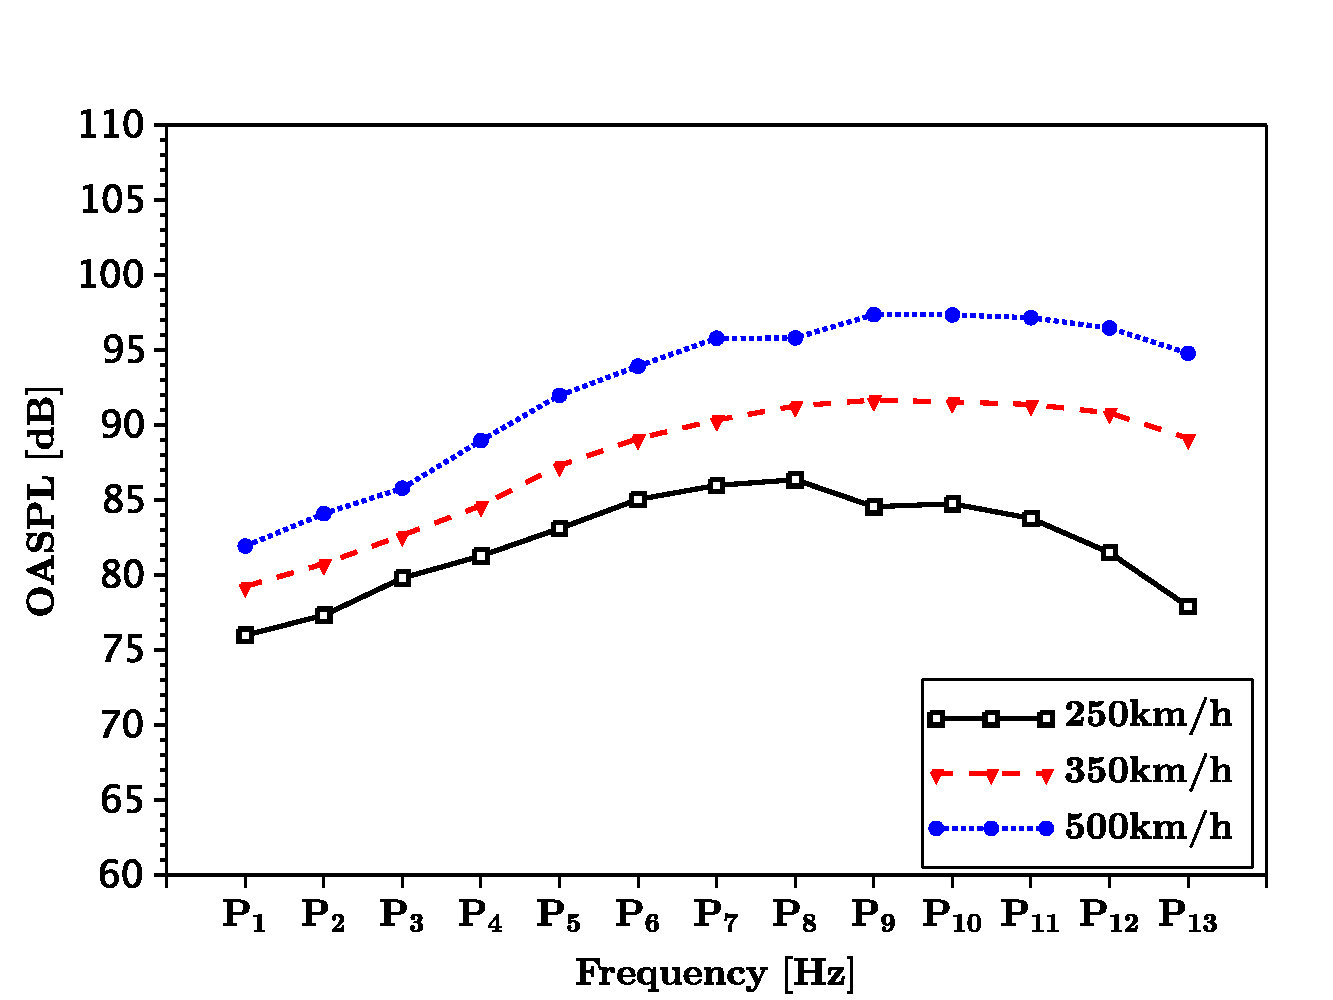
\includegraphics[width=\textwidth]{HC_OASPL_C}
                \caption{}
                \label{fig:HC_OASPL_C}
            \end{subfigure}%
            ~% add a small space
            \begin{subfigure}[b]{0.45\textwidth}
                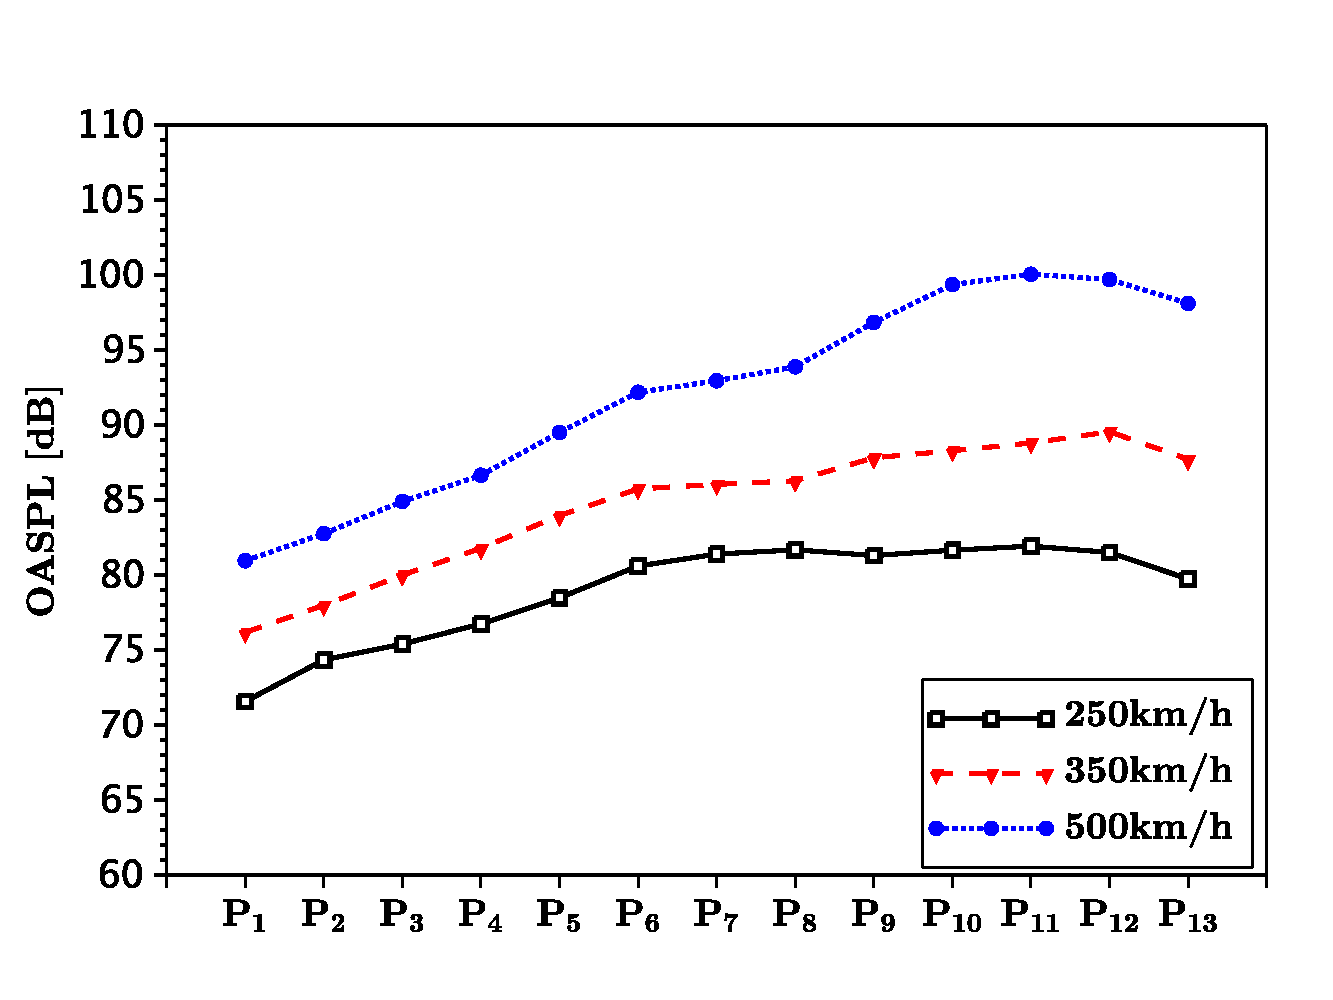
\includegraphics[width=\textwidth]{HC_OASPL_D}
                \caption{}
                \label{fig:HC_OASPL_D}
            \end{subfigure}%
            \caption{An Example for including multiple figures}
            \label{fig:HC_OASPL}
        \end{figure}
    \end{verbatim}
\end{center}
\begin{figure}[!htbp]
    \centering
    \begin{subfigure}[b]{0.45\textwidth}
        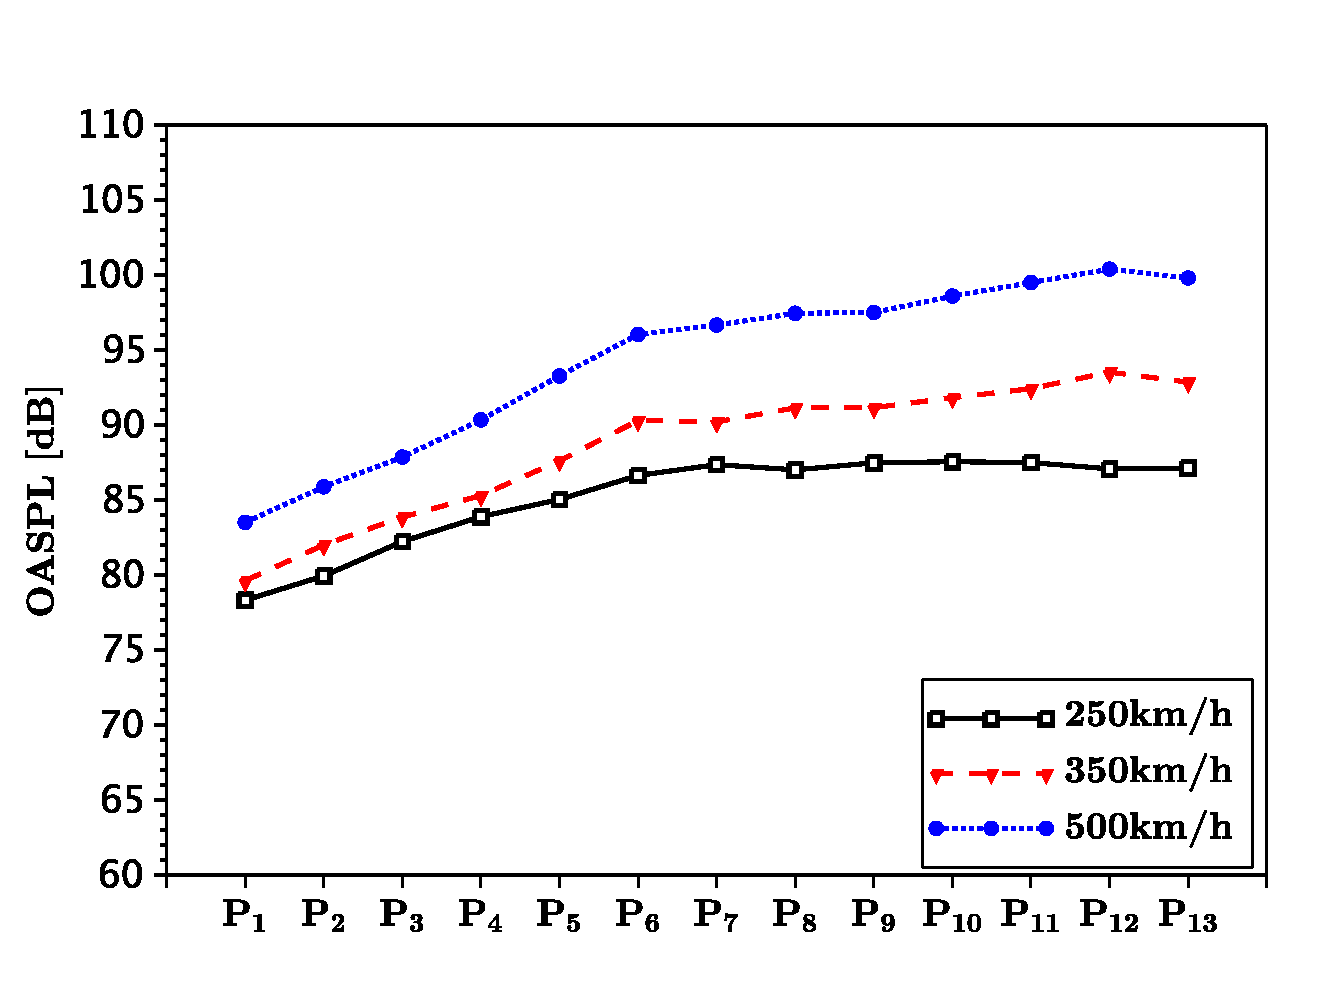
\includegraphics[width=\textwidth]{HC_OASPL_A}
        \caption{}
        \label{fig:HC_OASPL_A}
    \end{subfigure}%
    ~% add a small space
    \begin{subfigure}[b]{0.45\textwidth}
        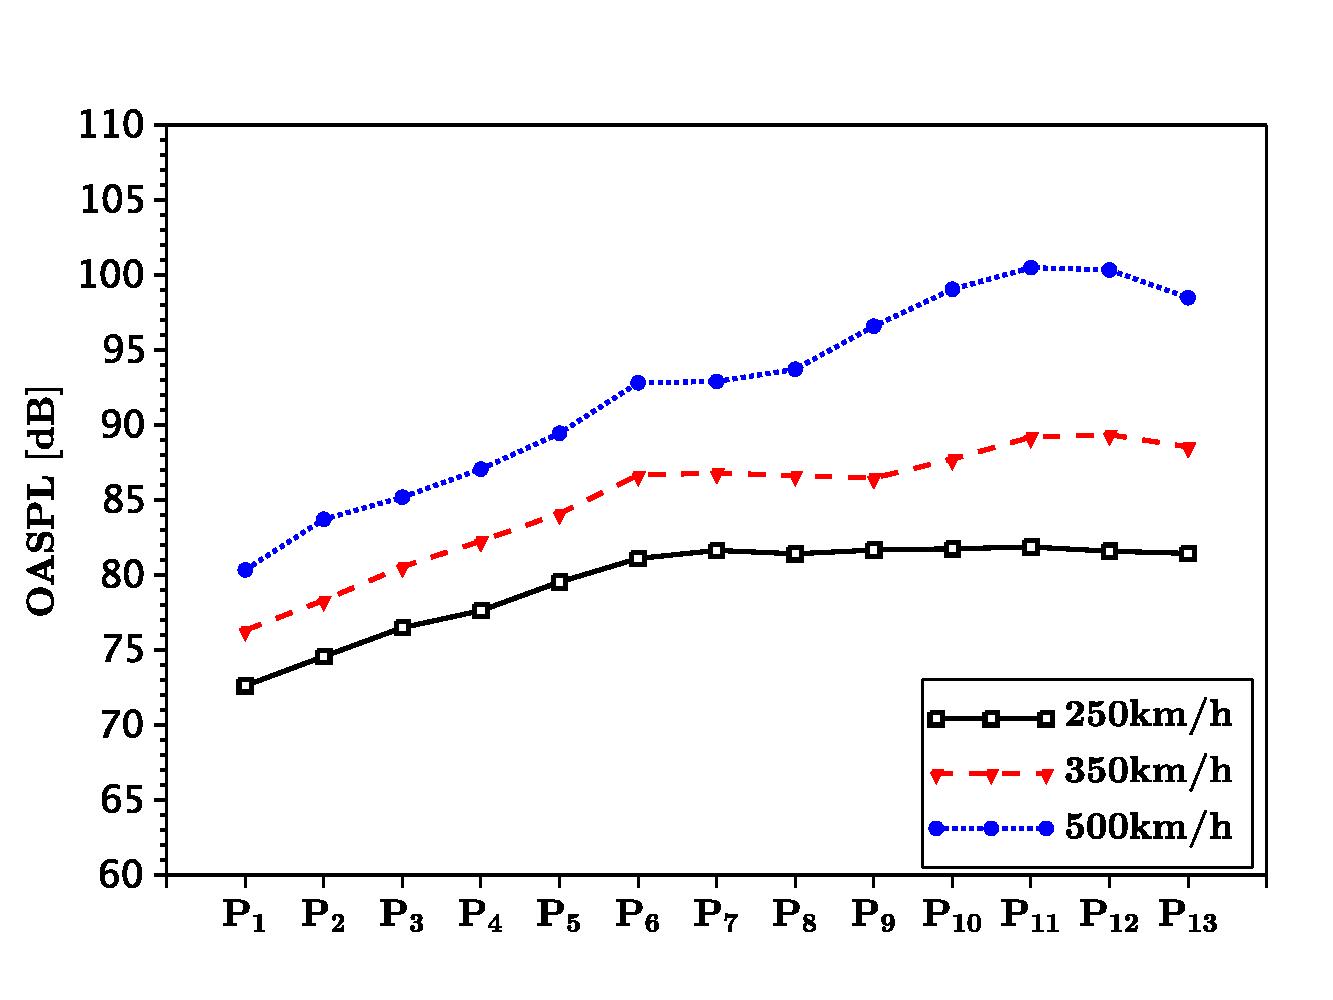
\includegraphics[width=\textwidth]{HC_OASPL_B}
        \caption{}
        \label{fig:HC_OASPL_B}
    \end{subfigure}%
    \\% change line
    \begin{subfigure}[b]{0.45\textwidth}
        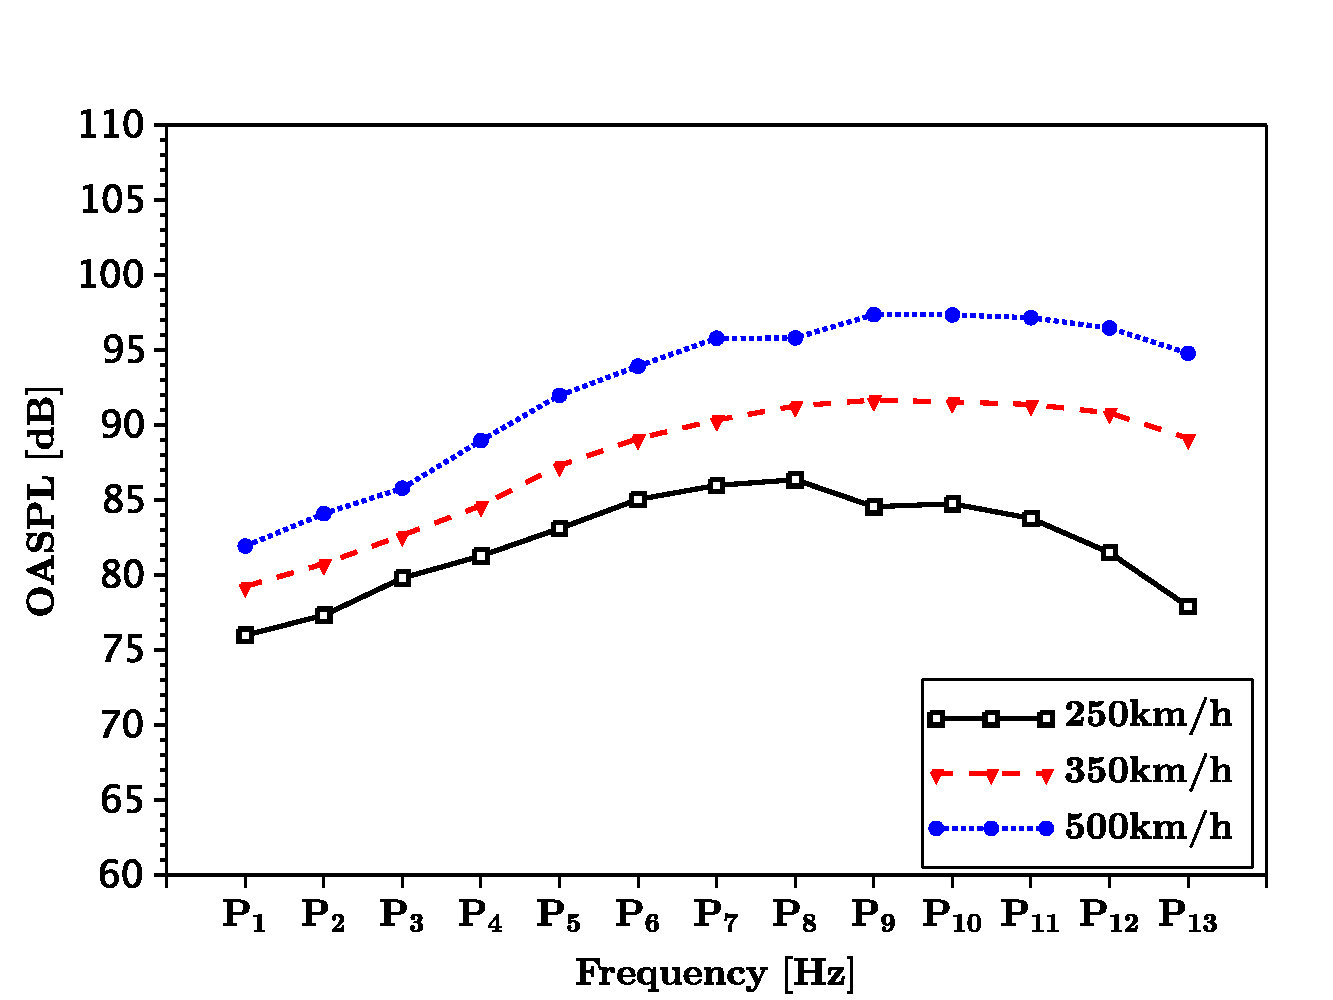
\includegraphics[width=\textwidth]{HC_OASPL_C}
        \caption{}
        \label{fig:HC_OASPL_C}
    \end{subfigure}%
    ~% add a small space
    \begin{subfigure}[b]{0.45\textwidth}
        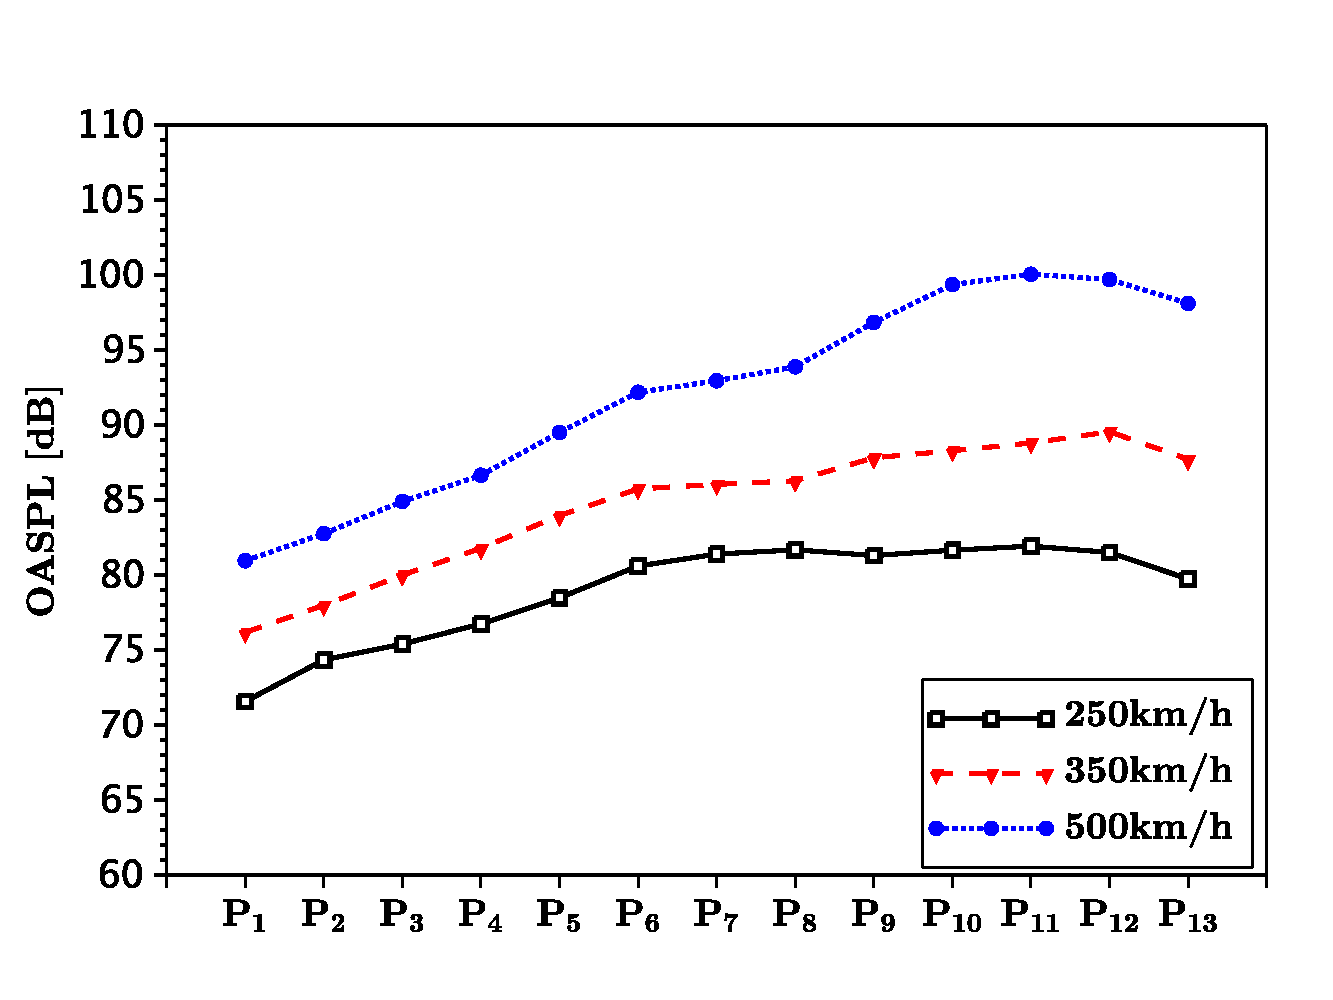
\includegraphics[width=\textwidth]{HC_OASPL_D}
        \caption{}
        \label{fig:HC_OASPL_D}
    \end{subfigure}%
    \caption{An Example for including multiple figures}
    \label{fig:HC_OASPL}
\end{figure}
% subsection Include Graphics (end)

\subsection{Include a citation} % (fold)
Suppose you are going to cite an article named "Document Preparation System", the procedures are:
\begin{itemize}
    \item Use Google Scholar search "Document Preparation System".
    \item Open "Cite" and choose "Import to Bibtex" under the target item.
    \item Copy the citation information of this article into the file "Myrefs.bib"
    \item Research dominant: cite this article by \verb+\citep{lamport1986document}+ like here \citep{lamport1986document}
    \item Citation dominant: cite this article by \verb+\citet{lamport1986document}+ like here \citet{lamport1986document}
    \item References list is generated automatically.
\end{itemize}
% subsection Include a citation (end)
\subsection{Generate nomenclature} % (fold)
In this template, a simple command for adding nomenclatures is provided. Therefore, packages for automatical nomenclature generation are not included. From my point of view, there is no need to use those packages and make things complicated. However, if you insist, there are a lot of available packages for creating nomenclatures. Recommended options are (Please Google the one you want to know):
\begin{itemize}
    \item listofsymbols
    \item nomencl
\end{itemize}
% subsection Generate nomenclature automatically (end)
% section How to use? (end)
